\documentclass{beamer}

% Preamble
\usepackage[utf8]{inputenc}
\usepackage{graphicx} 
\usepackage{amsmath} 
\usepackage{caption}
\usepackage{hyperref} 
\usepackage{xcolor} 
%\usepackage{fouriernc} %New Century Schoolbook with Fourier math

% Theme setup
\usetheme[secheader]{Madrid} 
\usecolortheme{beaver}

% Title page details
\title{Age from brain Data}
\subtitle{Project presentation}
\author{Marco Accerenzi}
\institute{Università di Pisa}
\institute[Università di Pisa]
{
  Dipartimento di Fisica
}
\date{\today}
\date[12 Settembre 2024] 
{Esame di Computing Methods for Exerimental Particle Physics and Data Analysis, 12 Settembre 2024}

\newcommand{\customSectionHeader}{
    \setbeamertemplate{section in head/foot}{}
    \setbeamertemplate{headline}{}
}



% Begin the document
\begin{document}

% Title Slide
{
    \customSectionHeader
	\begin{frame}
    	\titlepage
	\end{frame}
}

% Table of Contents
{
    \customSectionHeader
    \begin{frame}
        \title{Table of Contents}
        \tableofcontents
    \end{frame}
}

% First Slide
\section{Introduction}
\begin{frame}{Introduction to the project}
	The objective of this project was to develop a deep learning regression model, trained to predict the brain age of patients from data extracted from MRI scan of their brains. 

The model implemented in the project is capable of predicting the age of the patients in the data set with a RMS of about 6 years.

The best performing configuration for the model was a 2-hidden layer deep learning model, with 6 nodes per layer. The model trains and predicts at its best when the data is standardized and normalised using the methods provided in the project.

\end{frame}



% Second Slide
\subsection{Libraries}
\begin{frame}{Libraries}
    \begin{itemize}
		\item I used the \emph{keras} library for the regression model to write a problem specific implementation.     
		\item To read and manipulate the brain data, provided in .xlsx files, I used \emph{pandas}.
        \item For plotting the results and visualizations I used matplotlib.
        \item I used the \emph{os} and \emph{sys} modules from the python standard library to get and manipulate paths and directories.
    \end{itemize}
\end{frame}

% Third Slide
\subsection{What's in the code}
\begin{frame}{What's in the code}
The source code for this program contains several classes and some scripts, as to provide a framework to use the input MRI data from the ``raw'' excel file to produce a trained model capable of making predictions, evaluating and visualizing those predictions.
    \begin{itemize}
		\item The ExcelData class is responsible for reading the excel file and providing suitable input for the model.  
		\item The RegressionModel class contains the model itself. It implements methods for compiling, training, saving and loading regression models.
        \item The two ``Console'' scripts provide a basic UI to simplify the use of the project, allow the user to train a model and use it to make predictions without changing or writing any code.
    \end{itemize}
\end{frame}

% Third Slide
\begin{frame}{What's in the code 2}
    \begin{itemize}
        \item The Optimizator script allows to quickly choose values for the models hyper parameters.
		\item The Analysis script takes a .xlsx file containing the real labels and the predicted values to calculate the RMS and MSE of the predictions. It also allows to compare the data from the different groups in the original data set.
    \end{itemize}
\end{frame}

% Fourth Slide
\section{Data extraction and manipulations}
\subsection*{Data extraction}
\begin{frame}{Data extraction}
The MRI scan data for model training was provided for this project in the form of two .xlsx files, containing the features of 915 patients (or samples). For each sample the file also contains the real age at scan value (label) and the name of the group who provided the data for the sample (group name).
\begin{itemize}
\item Using the \emph{ read\_exce l} function provided by the\emph{Pandas} library the class creates a dataframe representing the data in the input file, including  the column labels. 

\item The \emph{ to\_numpy} method of the dataframe is then used to extract the numerical data to feed the model and is kept as a property of the ExcelData instace
\end{itemize}
All manipulations to the data is performed on copies of the \emph{numpy} array.

The samples can be shuffled before training to prevent overfitting, allowing to produce genuine predictions on the same test+validation data used in training.
\end{frame}

% Fourth Slide
\subsection{Data manipulations}
\begin{frame}{Data manipulations}

The ``raw'' data contains several blank cells and the various features have very different value ranges. To combat this issue the data is standardized and normalized. 

\begin{itemize}
\item As the excel file is read each blank cell is filled with a -9999 value. 
\item All columns of the array are normalized: each cell is divided by the max value of each column. In this calculation the cell containing a value of -9999 are excluded. 
\item The model will train itself to ignore the -9999 values. This allows the use of a larger data set compared to the one obtained by deleting all samples with a missing feature.
\item Normalisation and standardization greatly reduce the time needed for training. Instances of the model trained with normalized data make on average more accurate predictions on the data than instances trained without normalisation.
\end{itemize}

\end{frame}

% Fifth Slide 
\subsection{The effect of normalisation}
\begin{frame}{The effect of normalisation 1}
\centering
\begin{minipage}{0.48\textwidth}
	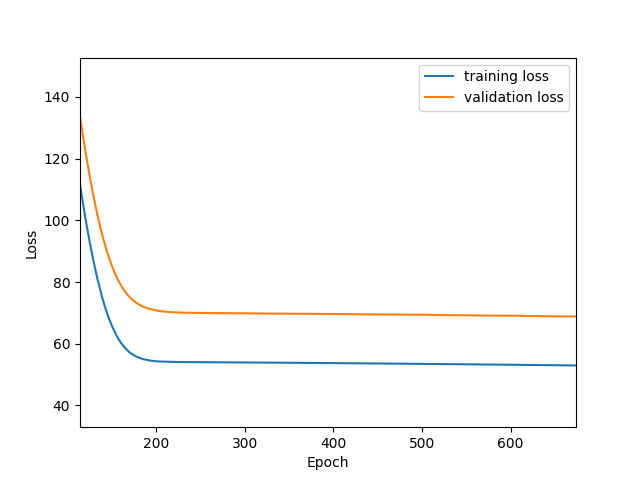
\includegraphics[width=\textwidth]{Figure_2.png}
	\captionof{figure}{Plot of the first training epochs using normalised data.}
	\label{historyNormalised}
\end{minipage}
\begin{minipage}{0.48\textwidth}
	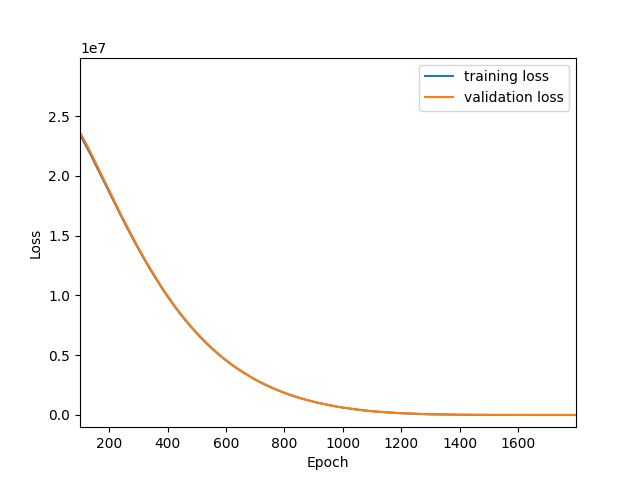
\includegraphics[width=\textwidth]{History_subplot_1.png}
	\captionof{figure}{Plot of the first training epochs using raw data.}
	\label{historyNonNormalised}
\end{minipage}

\end{frame}

% Sixth Slide 
\begin{frame}{The effect of normalisation 2}
\centering
\begin{minipage}{0.48\textwidth}
	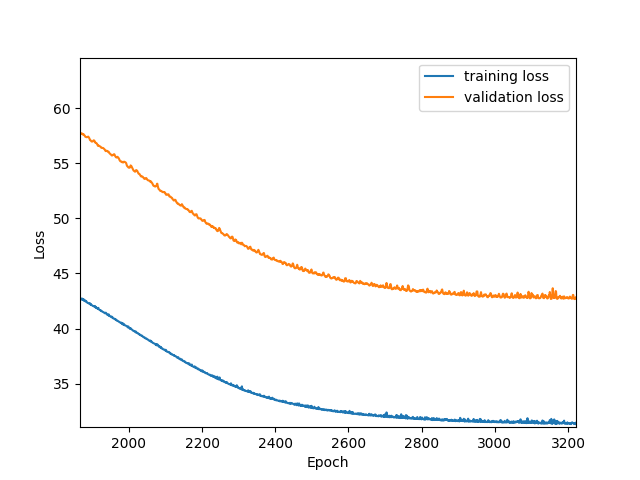
\includegraphics[width=\textwidth]{Figure_4.png}
	\captionof{figure}{Plot of the last training epochs using normalised data.}
	\label{historyNormalised2}
\end{minipage}
\begin{minipage}{0.48\textwidth}
	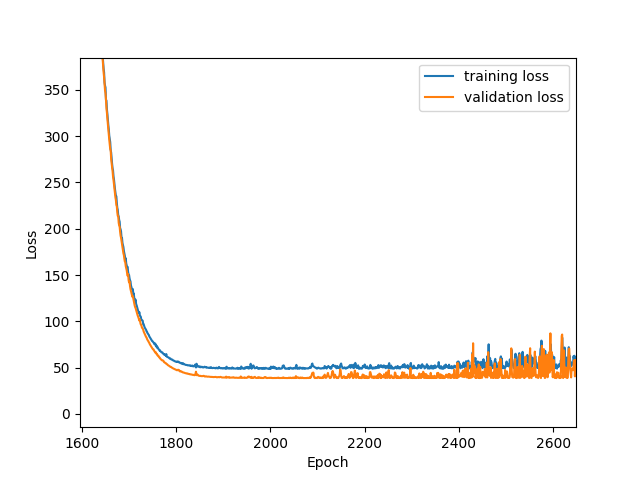
\includegraphics[width=\textwidth]{History_subplot_3.png}
	\captionof{figure}{Plot of the last training epochs using raw data.}
	\label{historyNonNormalised2}
\end{minipage}

\end{frame}

% Seventh Slide
\section{The regression model}
\begin{frame}{The regression model}
The regression model class uses the \emph{models}, \emph{layers} and \emph{callbacks} module from the \emph{keras} library.
It implements several methods:

\begin{itemize}
\item The Compile\_Model method defines the instance of the model, it sets up the layers and nodes of the model and fixes the shape of the input data. After the Compile\_Model method is called the model is compiled and ready for training.
\item The Start\_Training method trains the model over some data, using the supervised training algorithm provided by the \emph{keras} library. The number of epochs and other parameters of the training can be inputted by the user.
\item The Plot\_History and Save\_Model are meant to be used after Start\_Training, to save the training history and the model itself.
\item When initializing an instance of the model it's possible to use the \emph{load\_model} function to load a trained model: this model can be used only for inference and not for further training.
\end{itemize}

\end{frame}

% Eighth slide
\subsection{Callbacks}
\begin{frame}{Callbacks}
To optimize the training phase several callbacks are used:
    \begin{itemize}
        \item Early stopping:
			This callback stops training if, after a user-set number of subsequent epochs, the loss functions hasn't diminished. It allows to stop training before overfitting. After stopping it restores the best performing weights.
        \item ModelCheckpoint:
				This callback saves various ``checkpoints'' during training. It allows to keep a backup of the training progress.
        \item ReduceLROnPlateau:
				This callback reduces the \emph{learning rate} of the model if the training reaches a plateau (meaning if for a certain number of epochs the loss function stops diminishing). It reduces the amount by which the model's weights are changed during training, allowing for further training after reaching plateaus.
			\item PrintProgress:
				This is a modified version of Callback from the \emph{keras} library. It prints the loss functions every n epochs. The n parameter is set by the user through a ``verbose\_training'' parameter of the Start\_Training method.
    \end{itemize}
\end{frame}

% Ninth slide
\subsection{Optimizing the hyperparameters}
\begin{frame}{Optimizing the hyperparameters}
	The Optimizator.py script was used to choose the hyperparameters.

	It loops through several ``reasonable'' values of the hyperparameters and performs a shorter training run, the training history can then be evaluated by the user to choose the hyperparameters or to refine the Optimazator's range of parameters.

	The best performing model for this project was a 2-hidden layer model with 6 nodes per layer. This configuration had the fastest training time and overall the best average prediction performance.

\end{frame}

% Tenth slide
\section{Results and conclusion}
\begin{frame}{Predictions}

	The trained model was used to evaluate the input data and predict the ages of the patients.
Each training run produced slightly different models, the models trained with the optimal configuration have an average RMS of 7.1 years, the best performing model has a RMS of 6.30 years and a MSE of 39.66 over all the input data.

Repeated training could improve the average performance of the set of trained models but it is unlikely that these model could predict on the input data with a lower than 6 years RMS without gross overfitting. 

Only the best performing model will be considered for the next analysis.



\end{frame}

% Eleventh slide
\subsection{Comparing the results}
\begin{frame}{Comparing the results}

The performance of the model on all the different groups is compared in the figure below: the prediction error for the data of the ``Caltech'', ``MaxMun'' and ``SBL'' groups is vastly above the average. 

\begin{figure}
	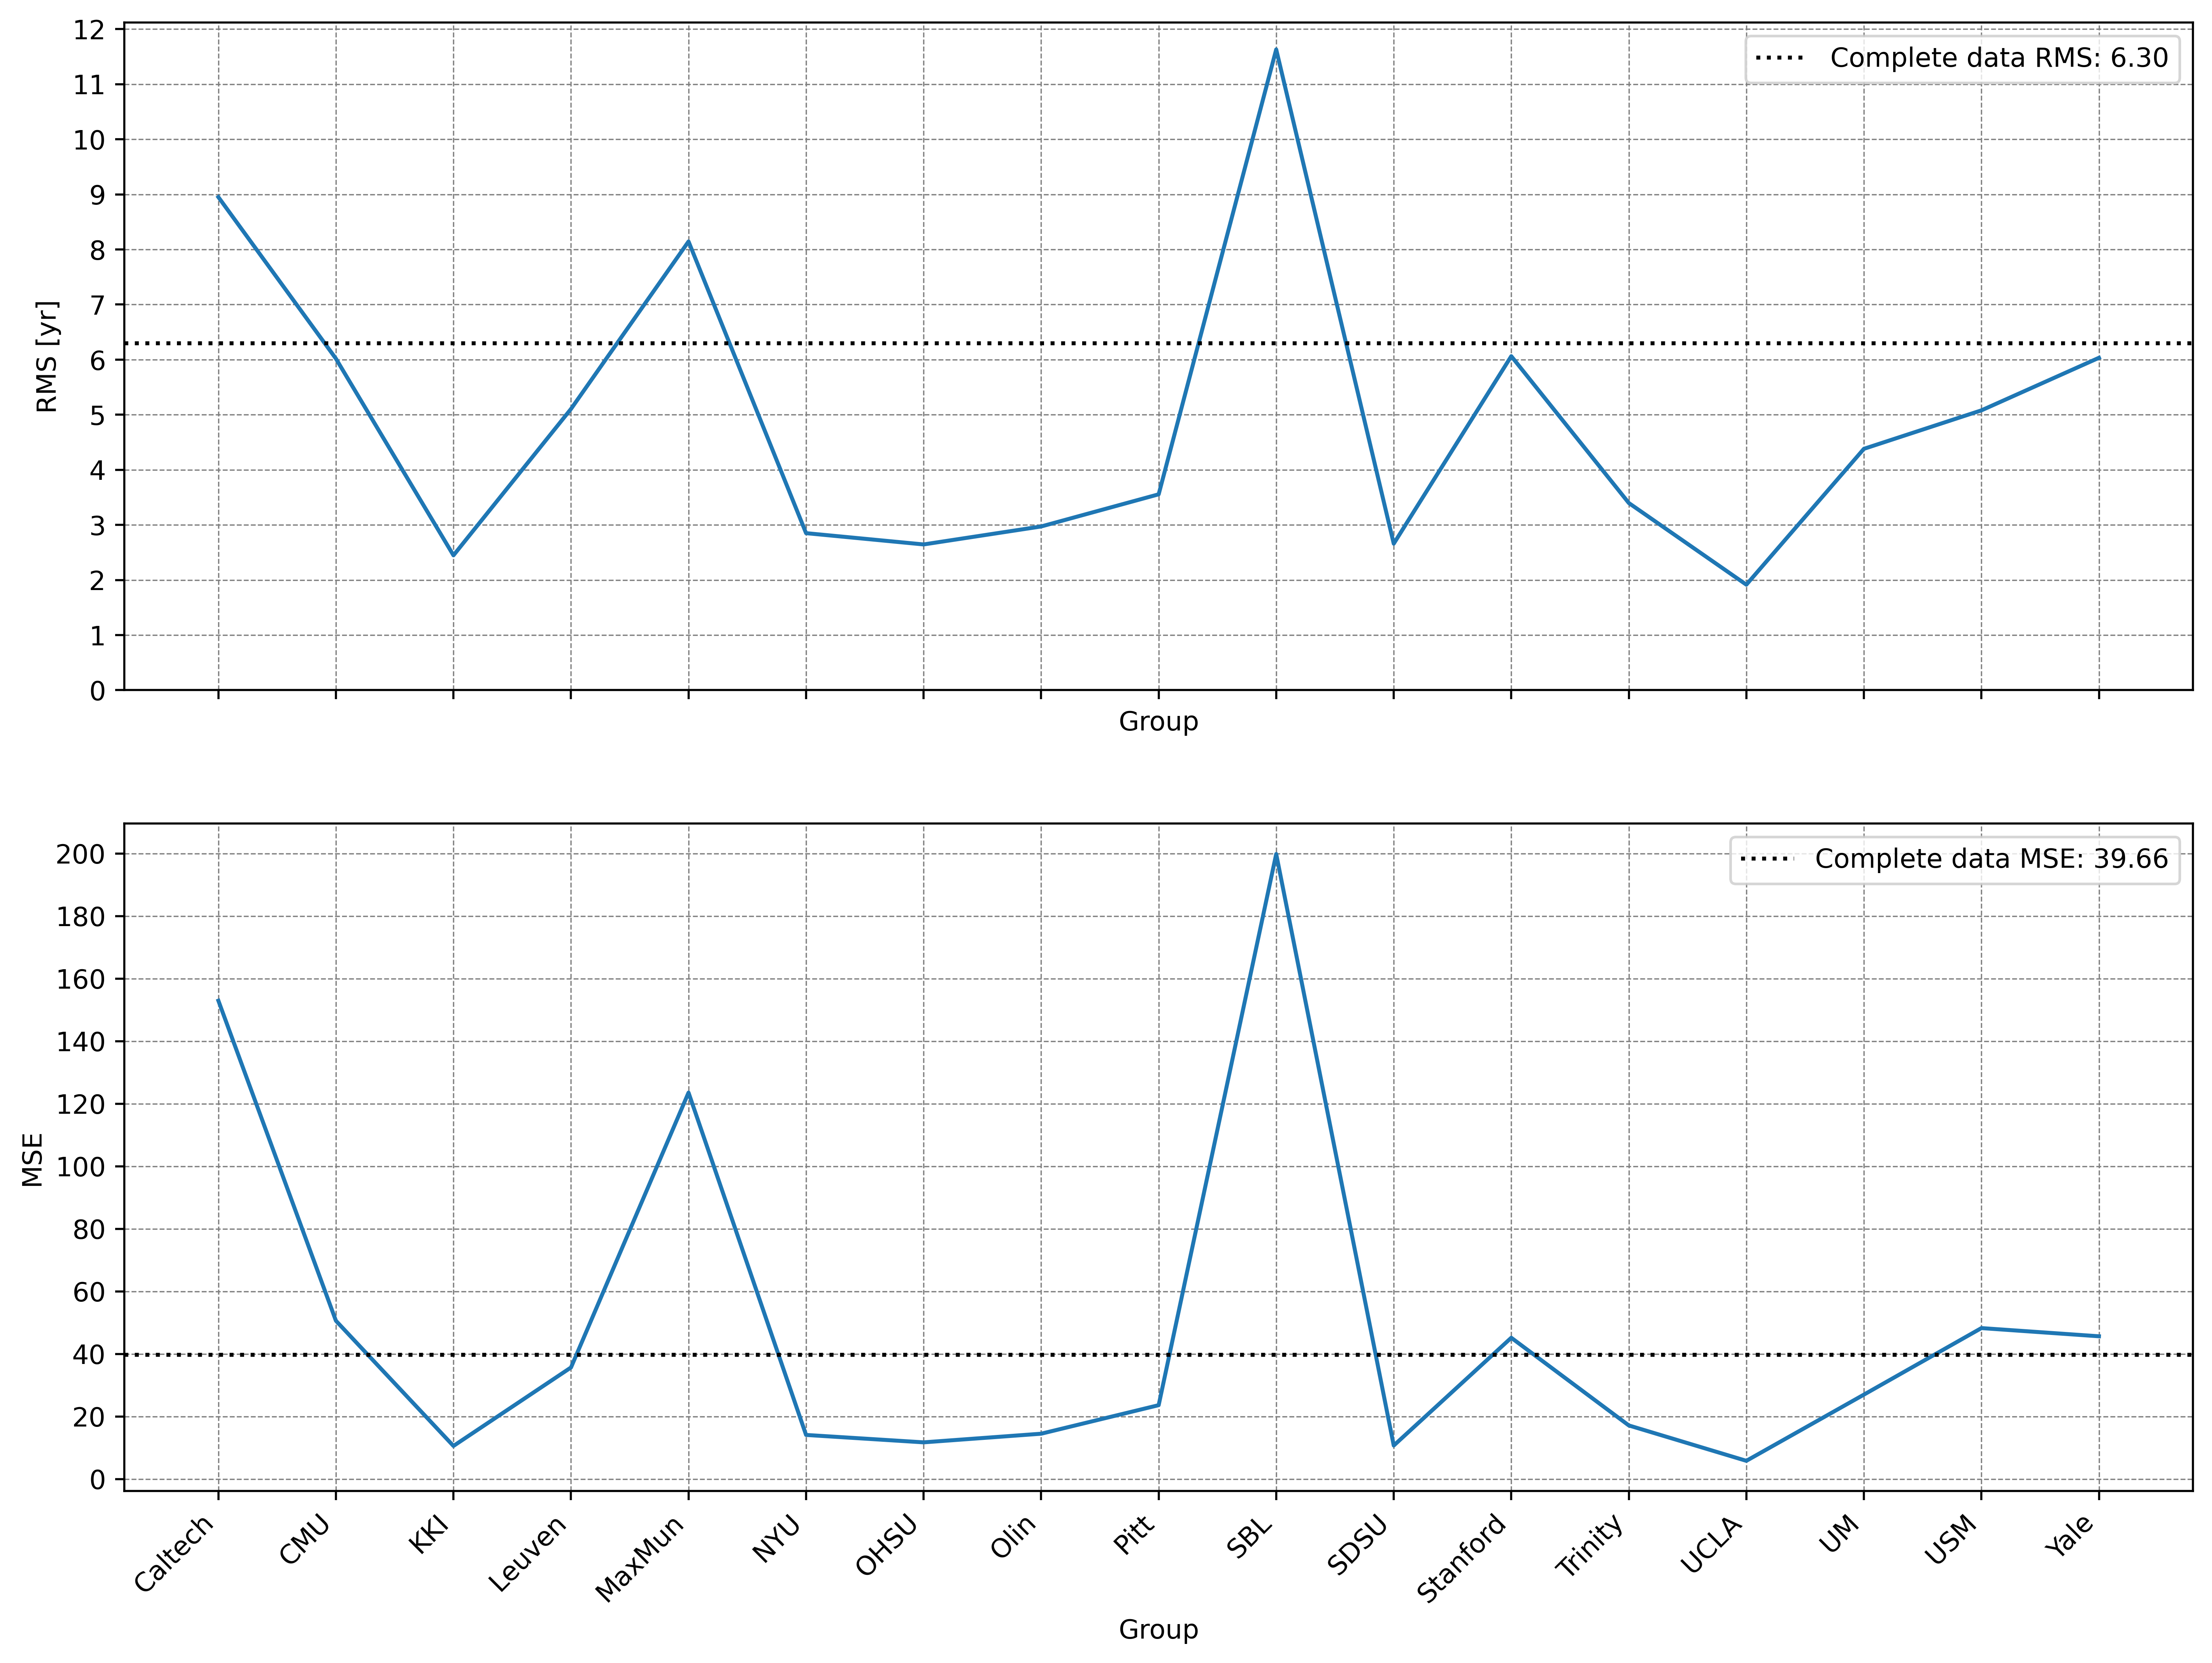
\includegraphics[width=0.65\textwidth]{result_1.png}
	\captionof{figure}{Plot comparing the prediction error for the various data groups. The error on the whole data set is displayed as a dotted line.}
	\label{plotRMSComparison2}
\end{figure}

\end{frame}


\begin{frame}{Comparing the results 2}

Repeating the training on a reduced data set by removing the three outlier data groups doesn't significantly improve the performance of the model: the trained model performs similarly on the remaining data groups but significantly worse for the three outliers. 

\begin{table}\centering
\begin{minipage}{0.45\textwidth}
	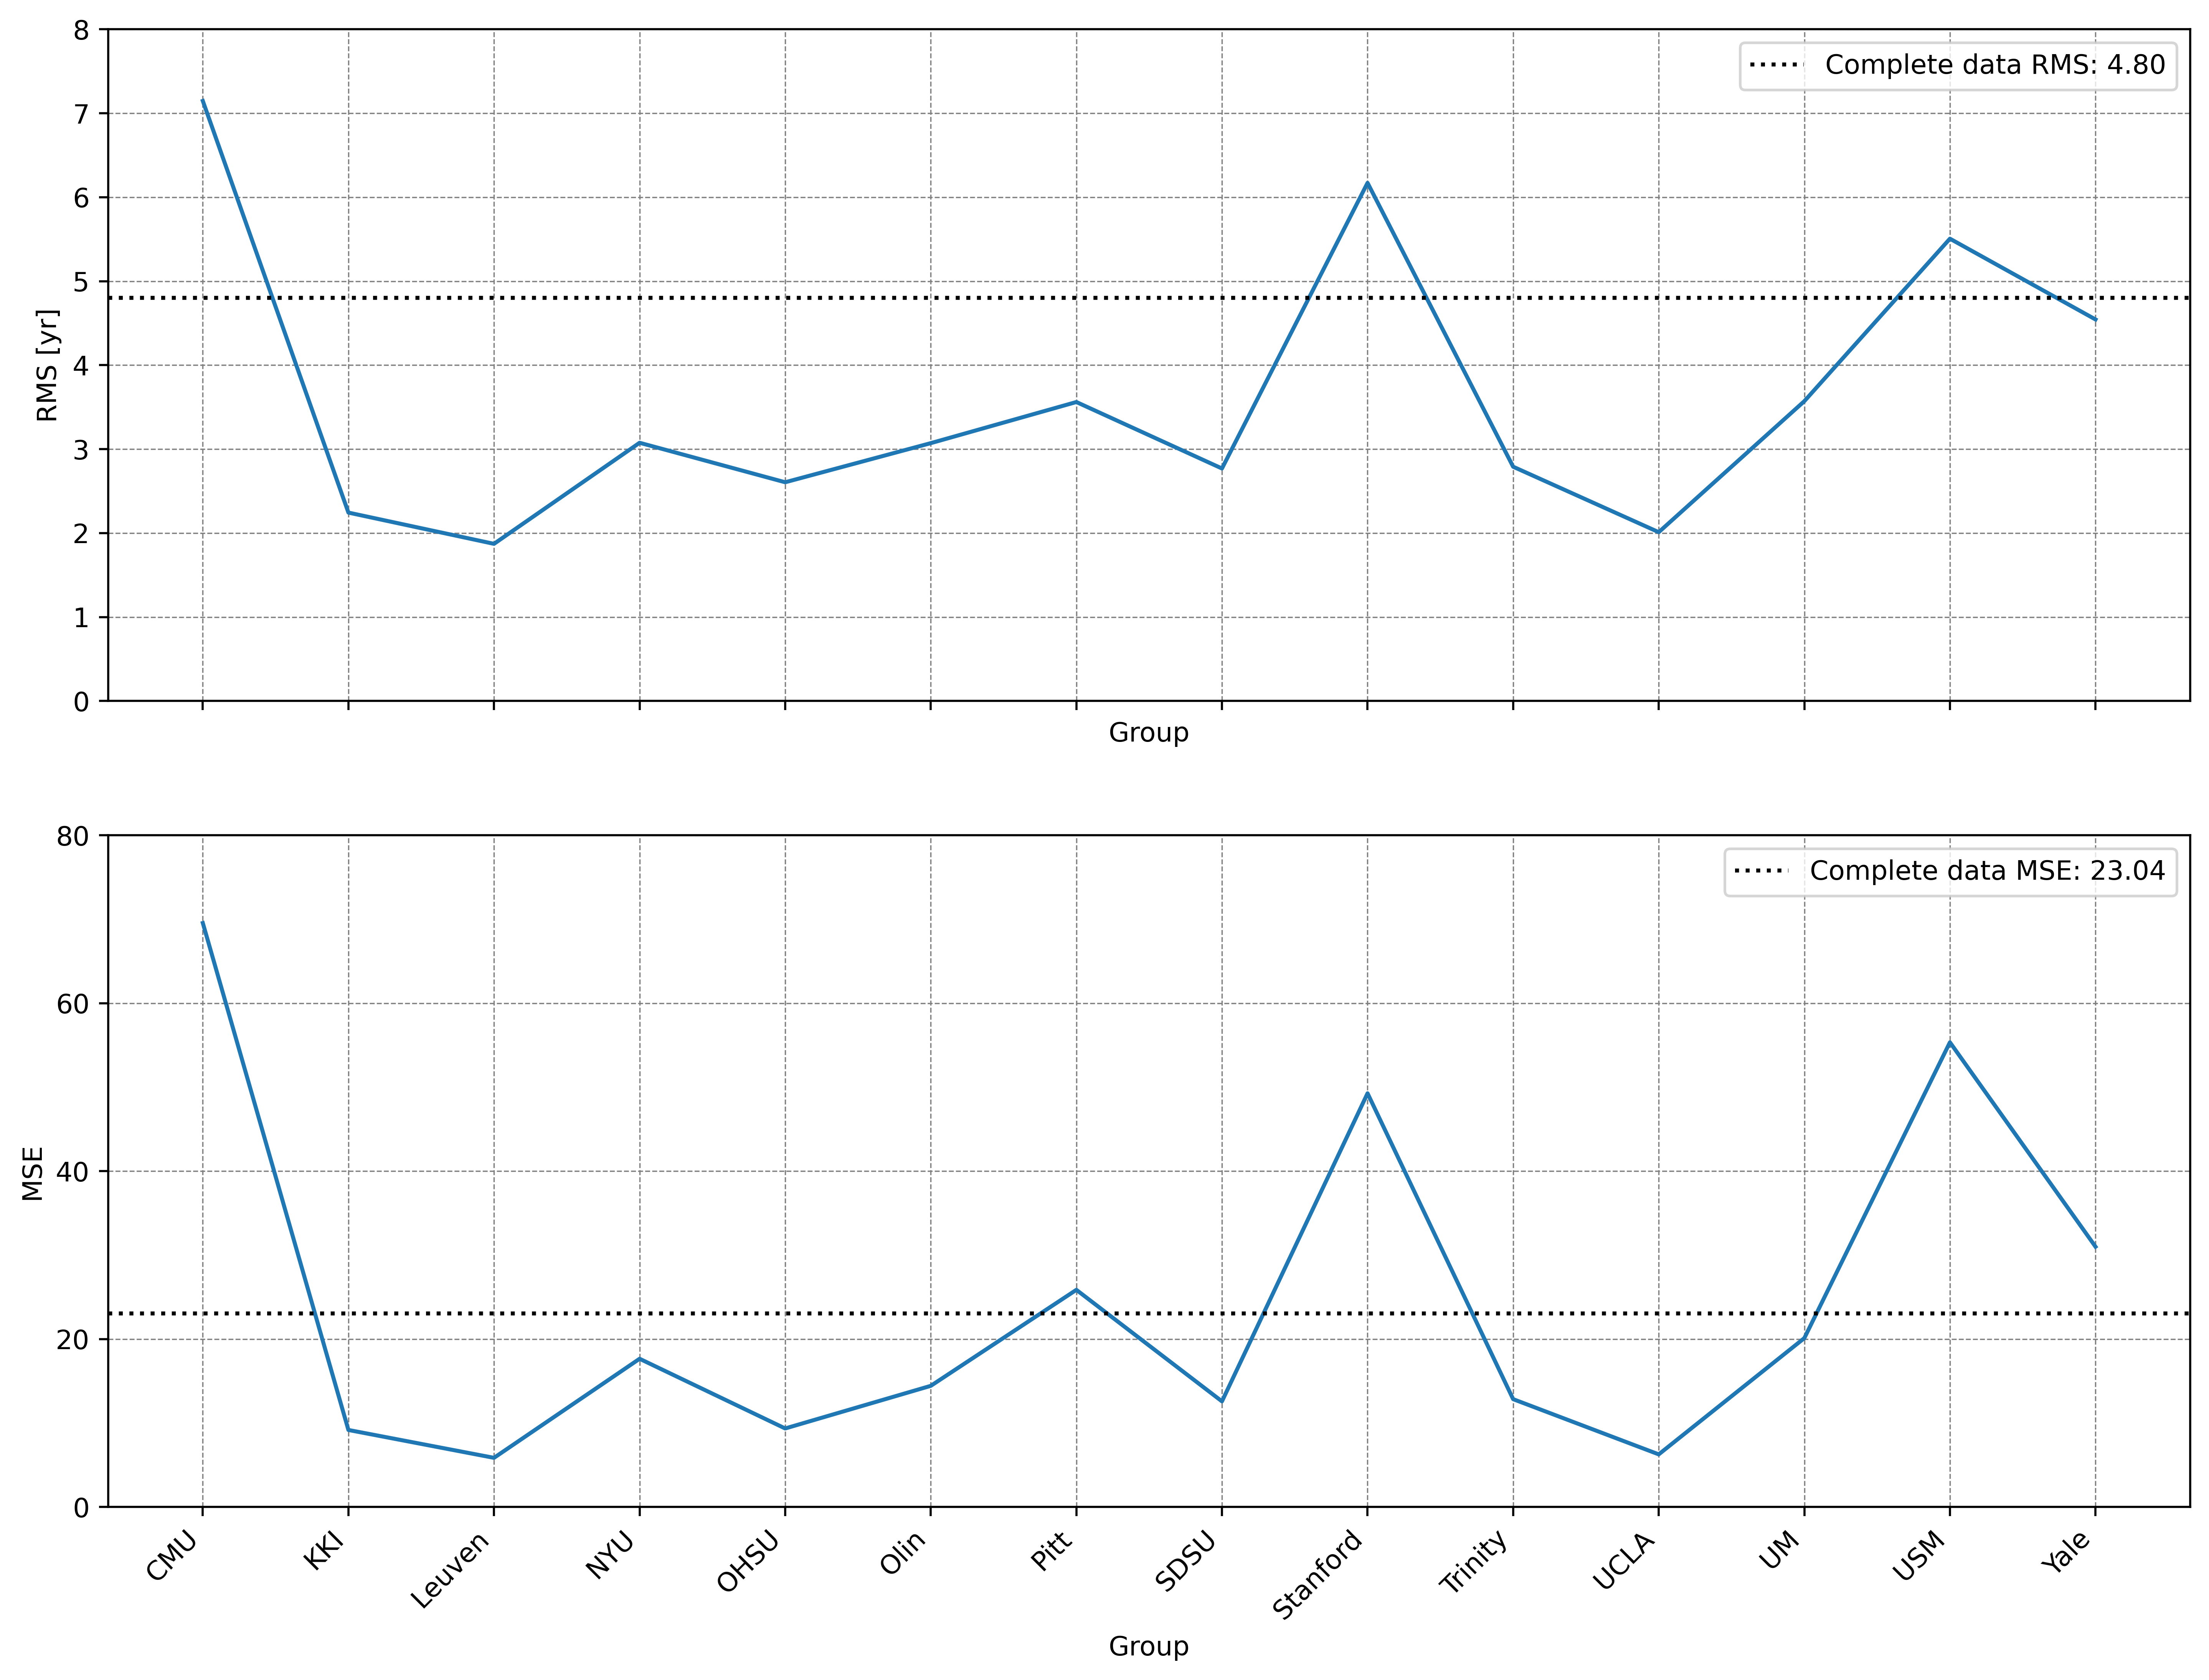
\includegraphics[width=\textwidth]{result_without_out.png}
\end{minipage}
\begin{minipage}{0.45\textwidth}
	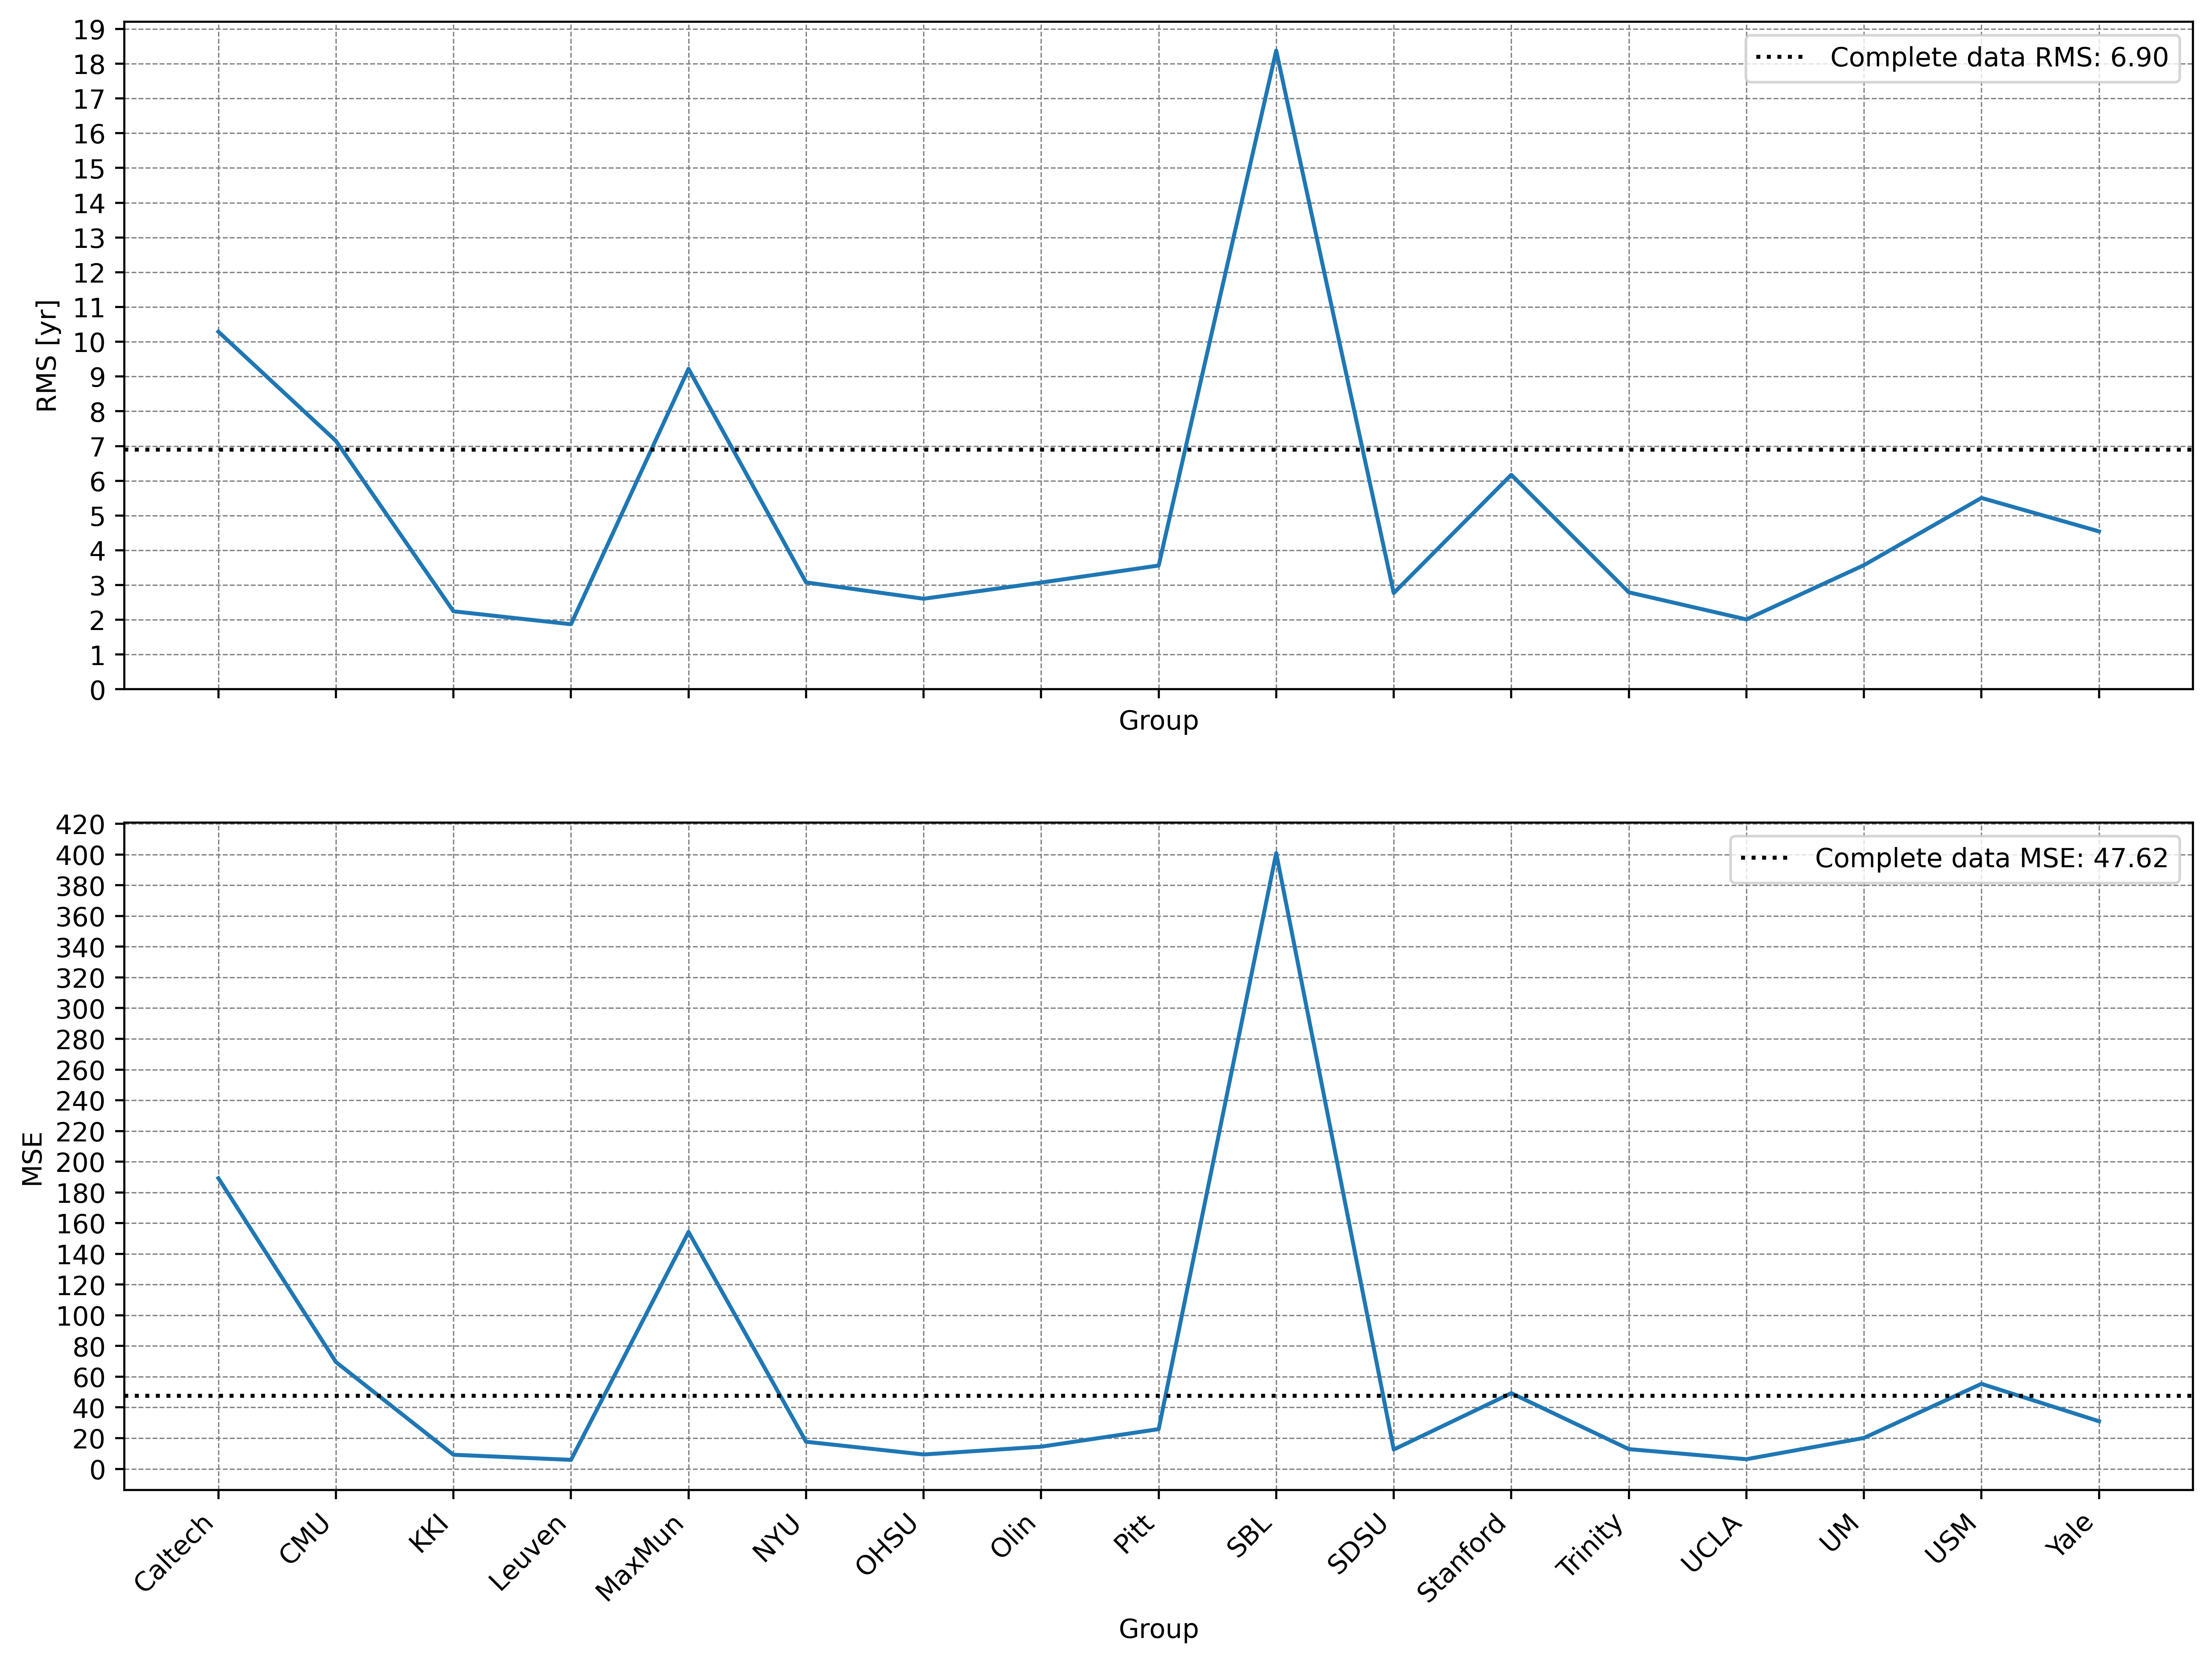
\includegraphics[width=\textwidth]{result_without_out_overall.png}
\end{minipage}
\end{table}

\end{frame}


% Backup slide 1

\begin{frame}{Git and the repository}

The project uses a public github repository. It has a main branch and three active branches: develop, feature/docs and feature/presentation.


\end{frame}

% Backup slide 2

\begin{frame}{Documentation}

The documentation for the project was generated via Sphinx, using its \emph{autodoc} functionality to extract the docstrings from the source code.

The public GitHub repository allows to distribute the projects documentation through ReadTheDocs and GitHub's own Pages.


\end{frame}




\end{document}
